\section{Výsledky numerického výpočtu hustoty stavov}
V tejto kapitole vyhodnotíme vzťah \eqref{eq:05rho_final} a výsledok prepojíme s teóriou Altschulera-Aronova, a porovnáme s experimentálnymi hodnotami. 

Ešte predtým ako urobíme finálny výpočet si musíme byť istý, že naša teória je správna. Vychádzame zo vzťahu \eqref{eq:05energy2}. Pri integrovaní cez $d\bar{y}$ zvolíme zatiaľ $\bar{y}_{max}=\infty$, teda nebudeme orezávať v recipročnom priestore. Naša nová teória musí byť konzistentná s už existujúcou teóriou pre self energiu Fockovej tienenej interakcie. Preto musí platiť
\begin{align}
\label{eq:06consistency}
\lim_{\tau\to\infty}\Sigma(E) = \Sigma_{screen}(E) \text{,}
\end{align}
kde $\Sigma_{screen}(E)$ je self energia Fockovej interakcie z rovnice \eqref{eq:fock_screen_final}.
 \begin{align}
  \label{eq:06fockscreen}
  &\Sigma_{screen}(\vec{k}(E))= \\ \notag
  &-\frac{e^2}{(2\pi)^2\epsilon_0} \biggl(
    \frac{k_F^2-k^2+k_s^2}{4k} \ln{\frac{(k_F+k)^2+k_s^2}{(k_F-k)^2+k_s^2}}-k_s\bigl(\arctan{\frac{k_F+k}{k_s}}+\arctan{\frac{k_F-k}{k_s}}\bigr)+k_F\biggr) \text{,}
 \end{align}
 kde za $k$ dosadíme vlnový vektor prislúchajúci danému $E$ v parabolickom disperznom zákone.
 
 Rovnosť \eqref{eq:06fockscreen} platí aj pri konečnom orezávaní, ale energia $\Sigma_{screen}$ musí byť rovnako orezaná. Preto pri výpočte hustoty stavov podľa 
 \eqref{eq:05rho_final} môžme počítať:                                      
 \begin{align}
 \label{eq:06densplot}
\frac{\rho(E)-\rho_0(E_F)}{\rho_0(E_F)}=\frac{d\Sigma_{\tau0}}{dE}-\frac{d\Sigma_{\infty}}{dE} \text{.}
 \end{align}

Funkcia \eqref{eq:06densplot} je náš finálny výsledok, ktorý prepojíme z Altschuler-Aronovovou teóriou a kvalitatívne porovnáme s experimentálnymi hodnotami. 
Altschuler-Aronovova teória v tomto tvare je 
\begin{align}
\label{eq:06altschuler}
\frac{\rho(E)-\rho(E_F)}{\rho(E_F)}= -\frac{1}{2\pi^3\hbar D l \rho_0(E_F)}+\frac{1}{\sqrt{2}(2\pi)^2(\hbar D)^\frac{3}{2}\rho(E_F)}\sqrt{|E-E_F|}
\end{align}

Pri vzťahu \eqref{eq:06densplot} ako aj teste konzistencie \eqref{eq:06consistency} využijeme obdĺžnikovú metódu integrovania:
\begin{align}
\int_a^b g(x)dx &\approx G(b)-G(a)\\
G(x) &= \sum_0^N \frac{g(x)-g(x+dx)}{2}\\
dx &= \frac{|a-b|}{N} \text{,}
\end{align}
kde $N$ je počet krokov.

V našom prípade za $g(x)$ dosadíme 
\begin{align}
g(x) = -\frac{e^2}{8\pi^4\epsilon_0 k_s^{-1}} \frac{\bar{y}^2}{1+\bar{y}^2}\sqrt{\frac{\epsilon_\tau}{E_F}}F(w,y)
\end{align}

Deriváciu self energie budeme tak isto počítať numericky a to z definície derivácie:
\begin{align}
\frac{df(x)}{d x} = \frac{f(x+\Delta x)-f(x-\Delta x)}{2\Delta x}
\end{align}

Pri numerických výpočtoch použijeme nasledovné hodnoty:

Náboj elektrónu $e = \SI{1.60217662e-19}{\joule}$, redukovaná Planckova konštanta $\hbar = \SI{1.0545718e-34}{\joule\second}$, hmotnosť elektrónu
 $m = \SI{9.109534e-31}{\kilo\gram}$, Fermiho vlnový vektor $k_F = \SI{1.6e10}{\per\meter}$, recipročná tieniaca dĺžka $k_s=k_F$, permitivita
 $ \epsilon_0 = \SI{8.854187e-12}{\farad\per\meter}$, doba života elektrónu $\tau_0 = \SI{6.58e15}{\second}$. Počet krokov integrovania $N=1000$
\begin{figure}[H]
\centering
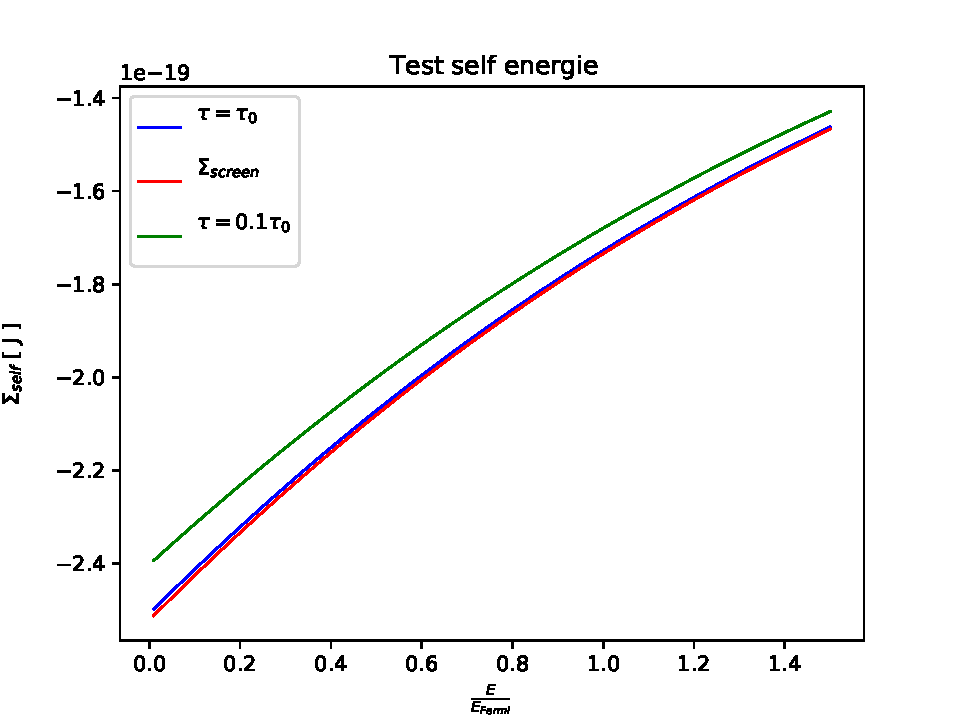
\includegraphics[scale=1]{grafy/plot_se_test}
\caption{Porovnanie self energie pre tienenú Fockovu interakciu so self energiou počítanou pomocou Thoulessovho ansatzu. Na x-ovej osi je bezrozmerná energia normovaná Fermiho energiou $\frac{E}{E_F}$, na y-ovej osi je self energia v jouloch.1 Za $\tau_0$ bola zvolená hodnota $\tau_0=\SI{6.58e-15}{\second}$ Z grafu je vidieť konzistentnosť podľa \eqref{eq:06consistency}.}
\label{fig:plot_test} 
\end{figure}

Z grafu na obrázku \ref{fig:plot_test} naša teória je konzistentná. V ďalšom počítame hustotu stavov podľa \eqref{eq:06densplot}, teraz už ale s konečným orezávaním (cut-off). Dá sa ukázať, že vhodný cut-off je
pre $q_{max}=\frac{1}{v_F \tau_0}$ resp. $\bar{y}_{max}=\frac{1}{v_F \tau_0 ks}$. Z týmto cut-offom vypočítame self energiu pre $\tau=\tau_0$ a pre $\tau=100\tau_0$ (postačujúca aproximácia nekonečného $\tau$) a dosadíme do \eqref{eq:06densplot}. 

\begin{figure}[H]
\centering
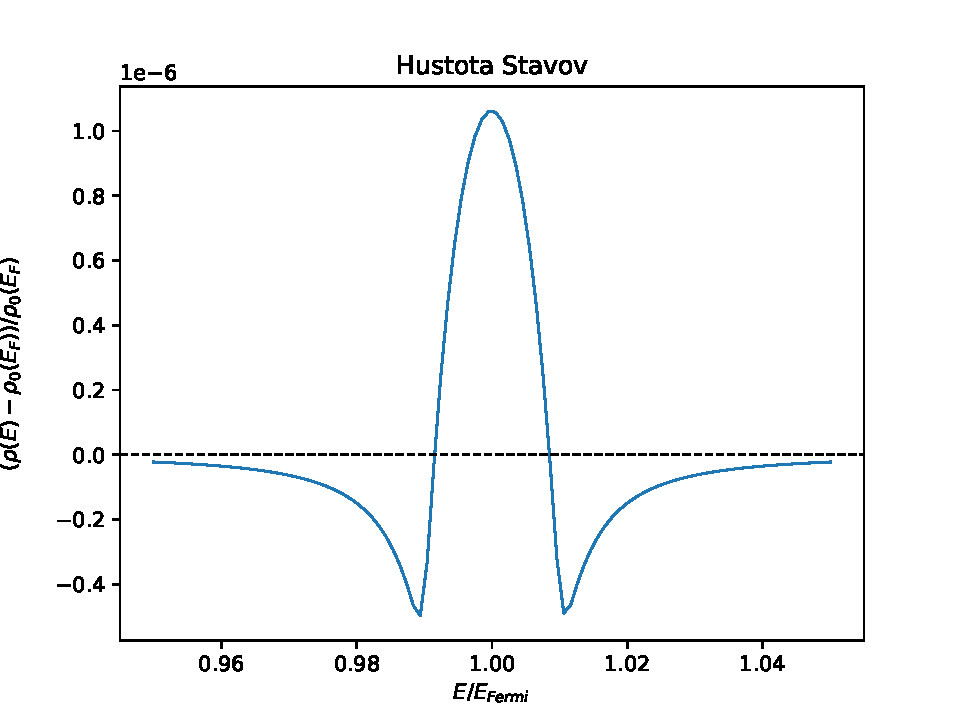
\includegraphics[scale=1]{grafy/plot_dos}
\caption{Hustota stavov podľa \eqref{eq:06densplot}. Na x-ovej osi je bezrozmerná energia, na y-ovej osi je hustota stavov podľa \eqref{eq:06densplot}.}
\end{figure}
Z grafu na obrázku je na prvý pohľad zrejmé, že nesedí s experimentom v blízkom okolí Fermiho energie. To sme však očakávali, pretože naša teória je pre energie ďalej od Fermiho energie. V okolí Fermiho energie máme k dispozícii Altschulera Aronova. 

 Našu teóriu z Altschuler-Aronovovou teóriou. Funkcie jednoducho "zošijeme" v bodoch kde krivka Altschulerovej hustoty stavov \eqref{eq:06altschuler} pretína našu krivku \eqref{eq:06densplot}, teda priebeh nebude hladký. Spojiť funkcie hladko je nad rámec tejto práce. V okolí Fermiho energie použijeme výsledok Altschuler-Aronova, a v bodoch ďalej od Fermiho energie použijeme náš výsledok. Pre ďalšiu analýzu výsledkov skúmame aj vplyv oboch členov \eqref{eq:06densplot} osobitne. Tak isto predvedieme aj vplyv druhého člena na štandardný postup pri výpočte hustoty stavov, teda spojenie Altschuler-Aronova s parabolickou hustotou stavov. Druhý $\rho_{corr}(E)=-\frac{d\Sigma_{\infty}}{dE}$  znamená zarátanie Fockovej tienenej interakcie.
\begin{figure}[H]
\centering
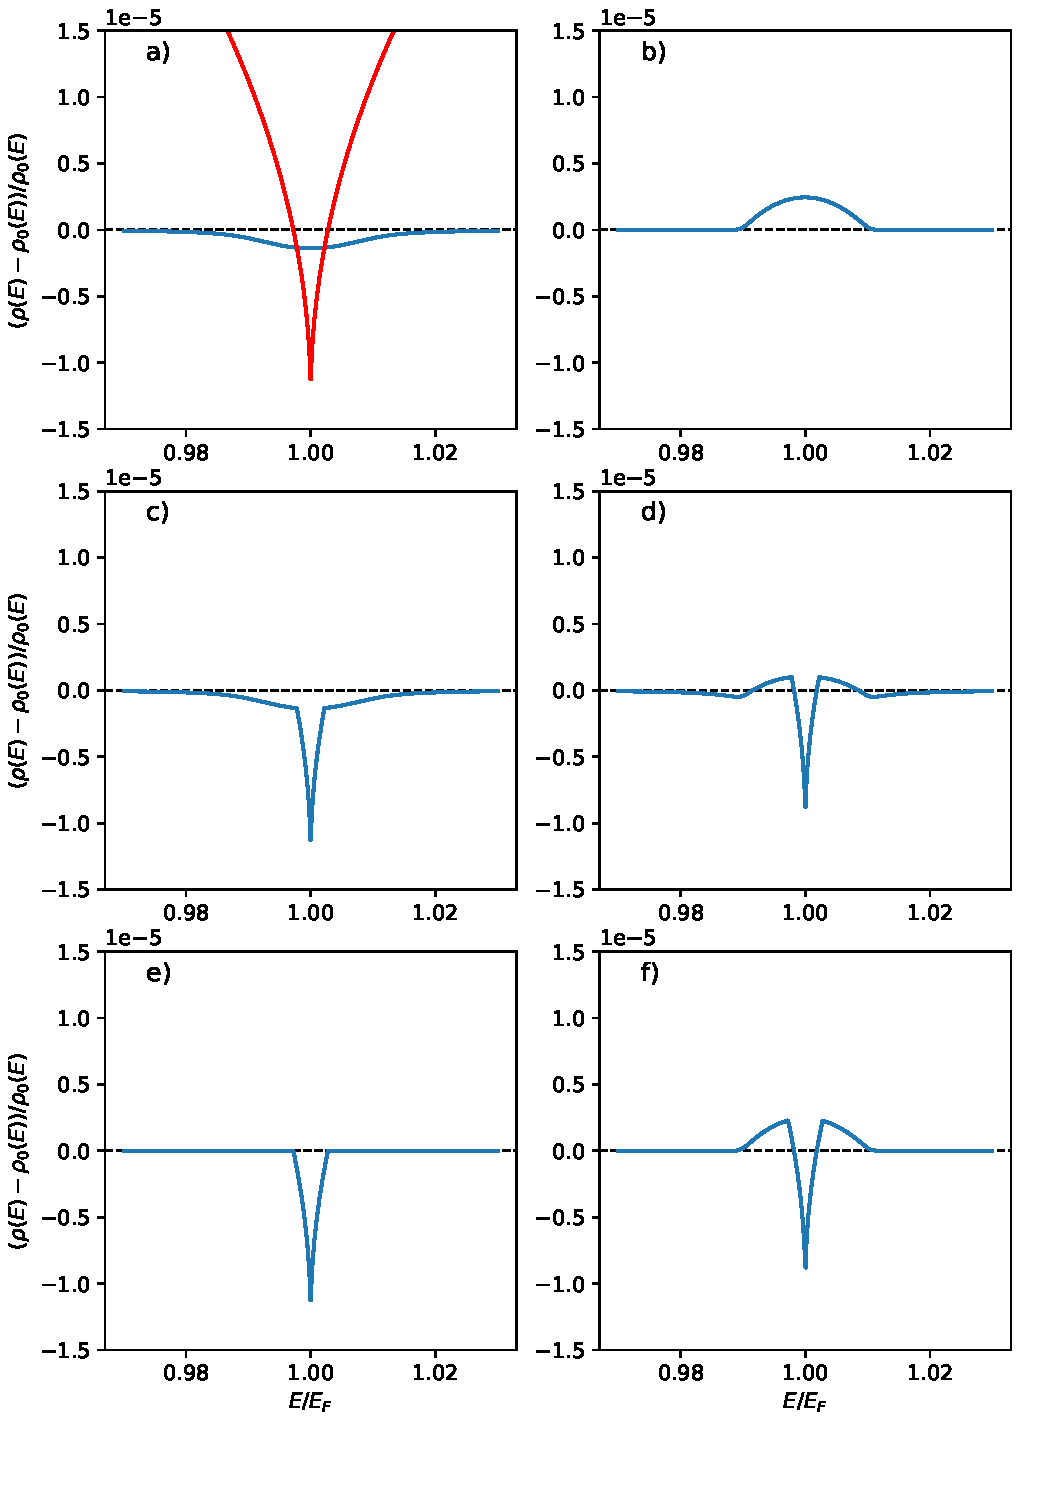
\includegraphics[scale=0.8]{grafy/plot_tau_1_c_1}
\caption{Analýza hustoty stavov. {\it a)} Altschuler-Aronov (červená čiara), prvý člen $\frac{d\Sigma_{\tau_0}(E)}{dE}$ {\it b)} druhý člen, $-\frac{d\Sigma_{\infty}(E)}{dE}$  {\it c)} Altschuler-Aronov spojený s prvým členom  \eqref{eq:06densplot}. {\it d)} oba členy \eqref{eq:06densplot} spojené z Altschuler-Aronovom. {\it e)} Parabolický disperzný zákon (čistý kov) spojený z Altschuler-Aronovom. {\it f)} Parabolický disperzný zákon spojený z Altschuler-Aronovom od ktorého je odčítaný druhý člen \eqref{eq:06densplot}}
\label{fig:results}
\end{figure}

Finálny výsledok je na obrázku \ref{fig:results} {\it d)}. Vidíme, že výsledok kvalitatívne pripomína experimentálne výsledky. Pozoruhodné sú hlavne dve lokálne maximá, ktoré pri štandardnom postupe nevidíme. Tieto maximá sú práve nahromadené stavy nad energiou $U_{co}$ z experimentu, ktoré spôsobia zvýšenie hustoty stavov oproti čistému kovu. 

Pozoruhodné je aj to, že maximá dostaneme aj vtedy, keď započítame iba druhý člen  $\rho_{corr}(E)=-\frac{d\Sigma_{\infty}}{dE}$ ako opravu hustoty stavov pre čistý kov doplnenú Altschuler-Aronovom.

Výsledky nám zatiaľ nesedia kvantitatívne s experimentom. Dajú sa však nafitovať menením $\tau_0$ a cutoffu $q_{max}$.
